\subsection{Cosmic Radiation Results}
\label{sec:Cosmic-Radiation-Results}

During the duration of the flight, a total of 16376 frames were collected and recovered successfully from the payload. Shown in Figure \ref{tracks} are a sample of tracks collected at float. The image in the upper left likely shows an interaction from a heavy ion while the rest of the tracks show a sampling of light and straight tracks. 


\begin{figure}[H]
	\begin{center}
	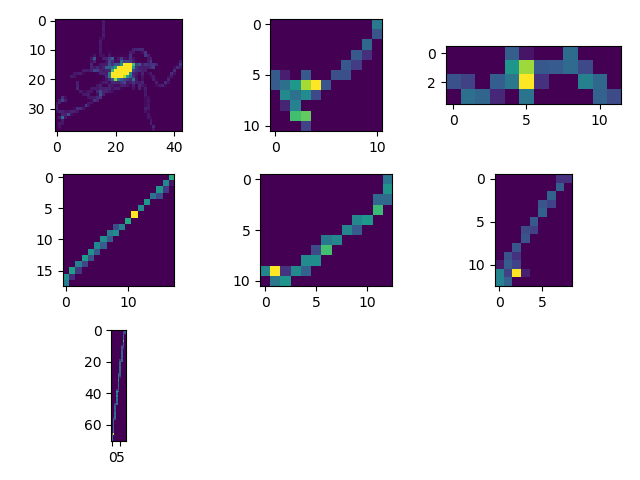
\includegraphics[width=0.75\textwidth]{figures/tracks.png}
	\caption{Tracks collected at float.}
	\label{tracks}
	\end{center}
\end{figure}

Shown in Figure \ref{let} (a) is the LET distribution for the entire population of tracks collected at float while \ref{let} (b) shows the LET distribution split up by track classification.

\begin{figure}[H]
\hfill
\subfigure[LET histogram from data collected during the duration of the flight.]{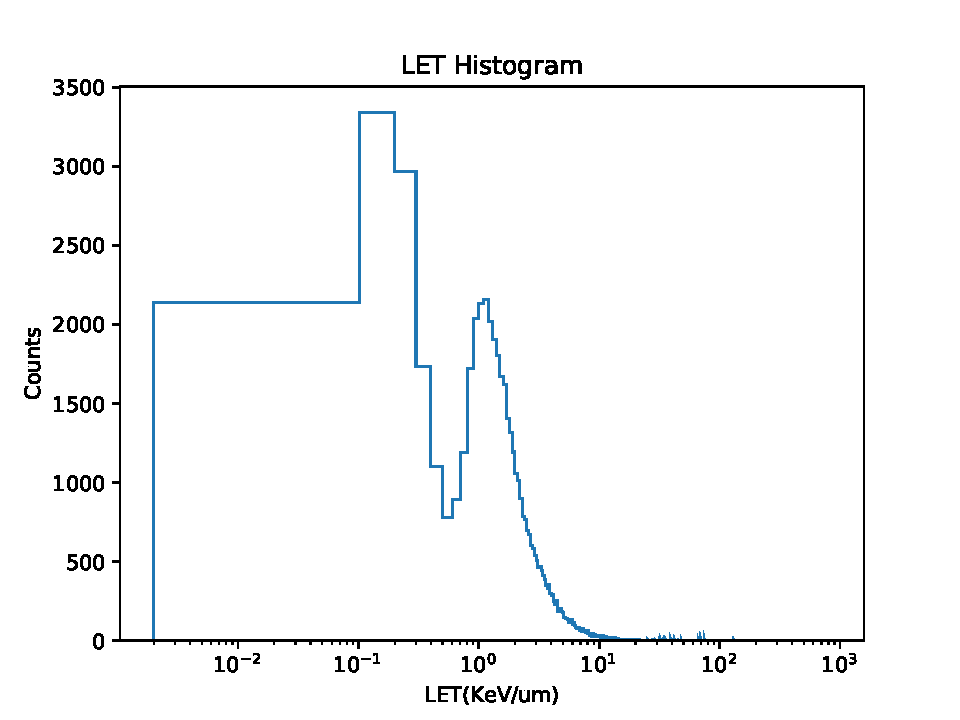
\includegraphics[width=8cm]{figures/LETSpectra2018.pdf}}
\hfill
\subfigure[LET histogram from each cluster type.]{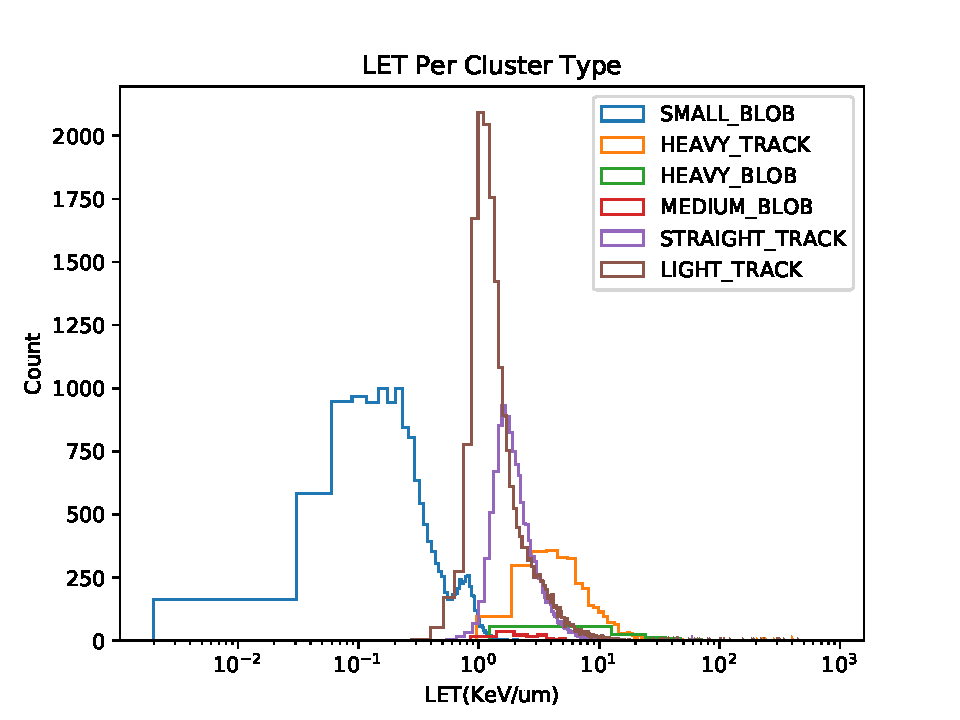
\includegraphics[width=8cm]{figures/LETSpectraPerCluster2018.pdf}}
\hfill
\caption{LET distributions data from Flight}
\label{let}
\end{figure}
\newpage

Shown in Figure \ref{counts} is a comparison of the count rate for the SORA 2017 and 2018 flight. The shape of the data is nearly identical however one can observe that the 2018 flight has a higher variability and is slightly less homogeneous when compared to the 2017 data. The overall variability is due to a faster frame rate and the period of decreased variability that occurs just after the peak is due to a test of the ability to dynamically modify the frame rate via uplink commands. Another significant feature of the data is that the 2018 flight appears to be shifted upwards by approximately two counts per second when compared to the 2017 data. This would seem to suggest a higher flux during the 2018 flight.
\begin{figure}[H]
\hfill
\subfigure[Counts from data collected during the 2017 flight.]{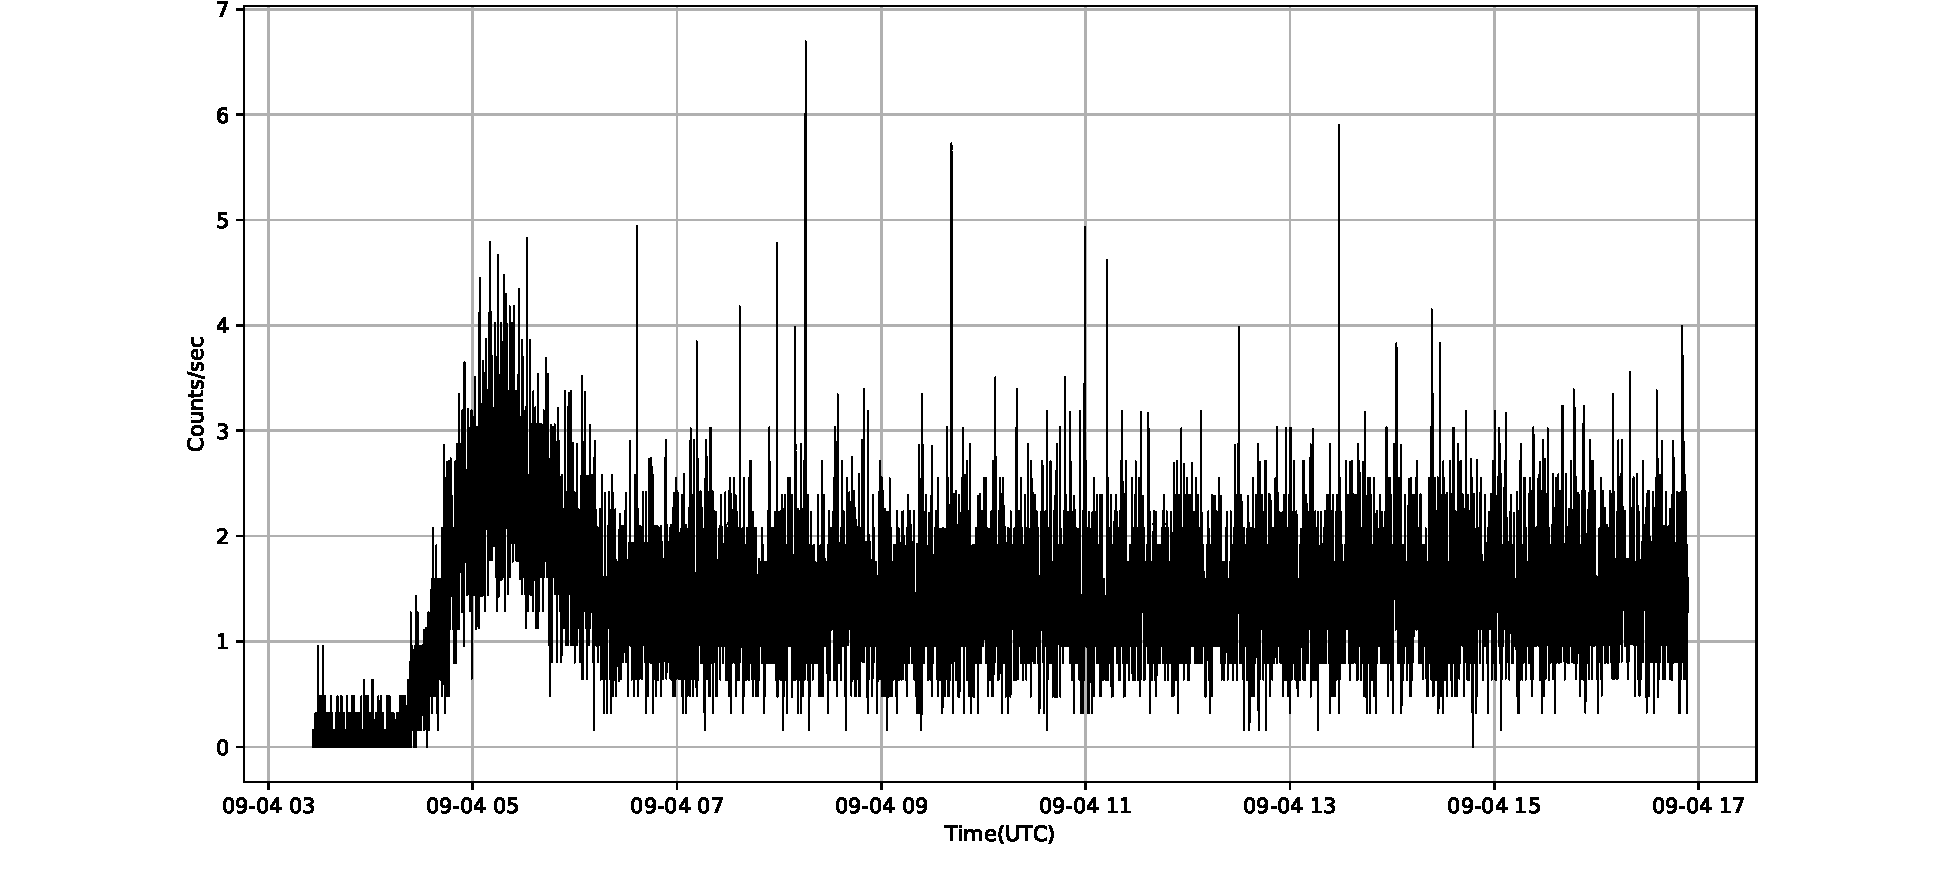
\includegraphics[width=\textwidth]{figures/counts_per_second_2017.pdf}}
\hfill
\subfigure[Counts from data collected during the 2018 flight.]{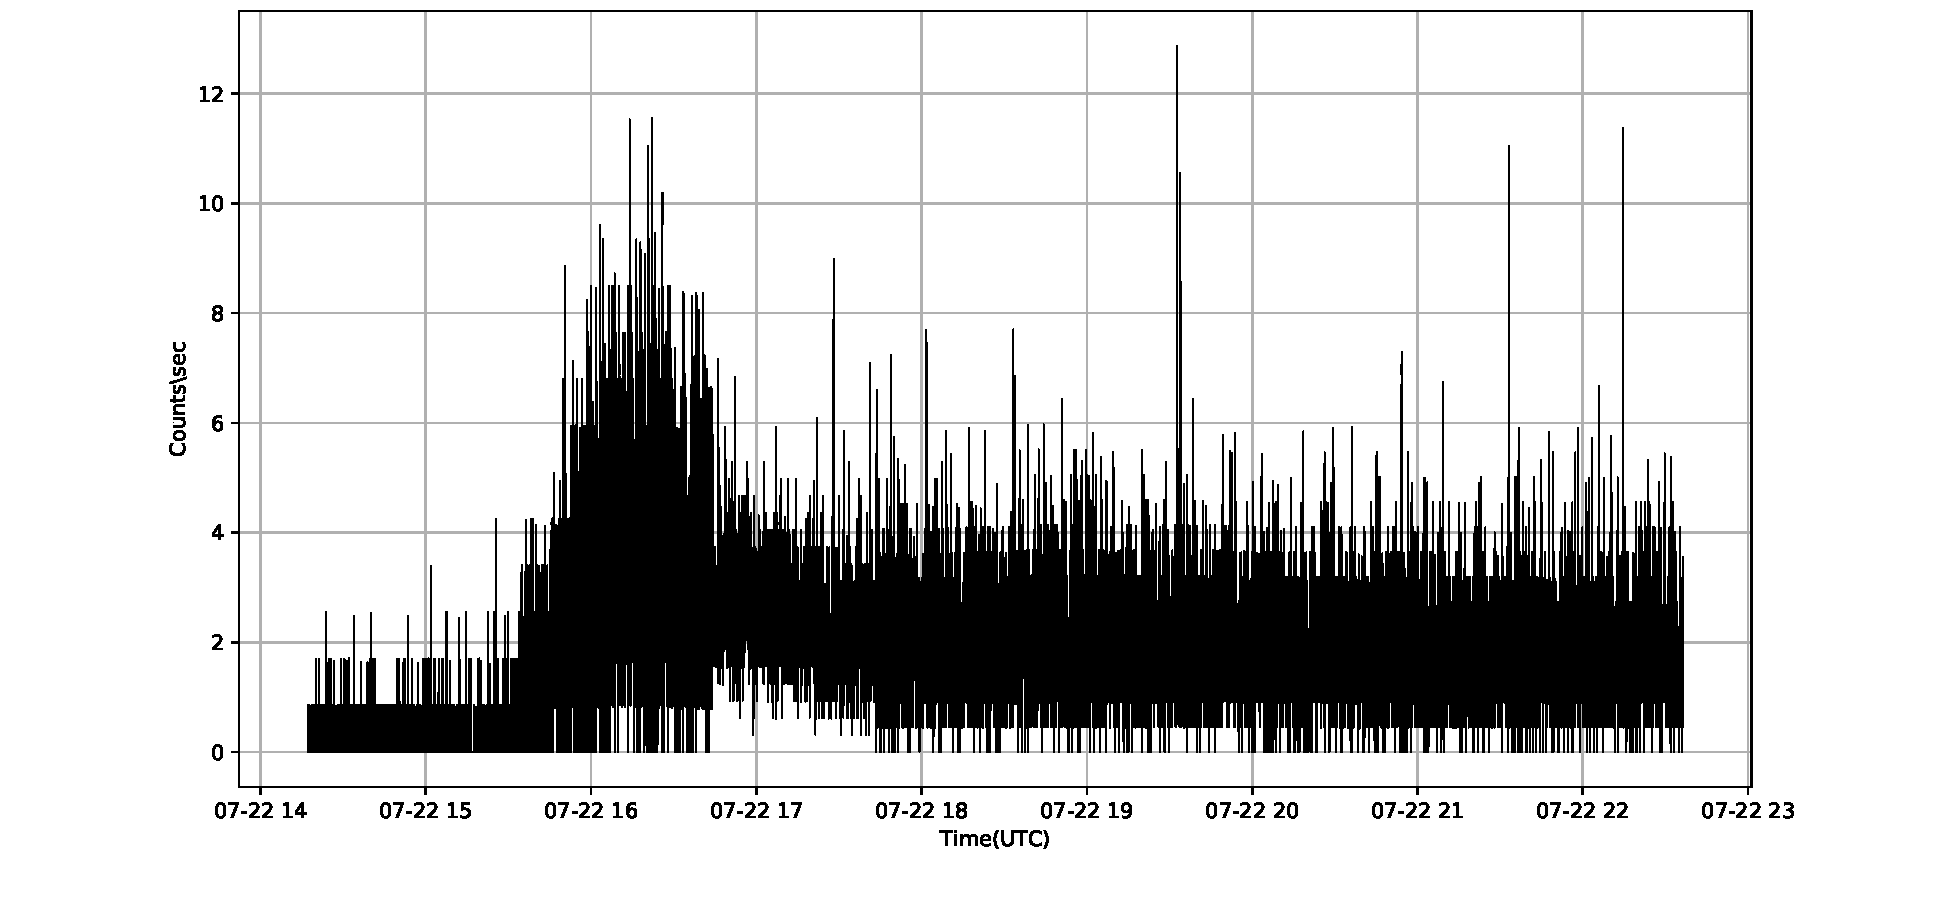
\includegraphics[width=\textwidth]{figures/counts_per_second_2018.pdf}}
\hfill
\caption{Cluster counts data from Flights 2018 and 2017}
\label{counts}
\end{figure}

